\section{Forecasts}

\subsection{Optimising Design Variables}

In order to find the best experimental set up and quanitify the improvement from stage-2 to stage-3 or stage-4, I used the mock covariances as described in section 3.3. By varying one experimental variable at a time and holding the rest fixed, I was able to forecast the minimum experimental uncertainty on the PMF strength, $\sigma(B_{1Mpc})$ for each mock experiment and plot the relationship between $\sigma(B_{1Mpc})$ and the experimental variables.

While varying the experimental design, the fixed values need to be chosen with care. The choice of values will determine how reliable the following forecasts are. The values I chose for the variables are more characteristic to stage-3 experiments than stage-4 ones. The average survey area of a stage-3 experiment is of the order $\sim$10 000 square degrees (roughly one quarter of the sky). On the other hand, stage-4 experiments are expected to achieve approximately half-sky coverage. Since I chose the stage-3 expected sky coverage, we can expect that the forecasts will underestimate the accuracy gains for stage-4 experiments. On the whole, the values I chose reflect the design specifications of a stage-3 experiment so we would expect the forecasts for stage-4 improvements to be conservative. Table 3 shows the values chosen for a variable when it was held fixed.

\begin{table}[h]
\centering
\caption{Fixed Variables}

\label{my-label}
\begin{tabular}{l|l}
\multicolumn{1}{c}{Variable} & \multicolumn{1}{|c}{Value} \\ \hline
\multicolumn{1}{c}{Survey area $(deg^2)$} & \multicolumn{1}{|c}{10313}  \\
\multicolumn{1}{c}{Noise ($\mu$K arcmin)} & \multicolumn{1}{|c}{1.9}   \\
\multicolumn{1}{c}{$\ell_{knee}$} & \multicolumn{1}{|c}{100} \\
\multicolumn{1}{c}{beam width (arcmin)} & \multicolumn{1}{|c}{4.0}   \\
\multicolumn{1}{c}{calibration error (\% error)} & \multicolumn{1}{|c}{0.01} \\
\multicolumn{1}{c}{beam uncertainty (\% error)} & \multicolumn{1}{|c}{0.05}
\end{tabular}
\begin{flushleft}
This table shows the values I chose for each independent variable when they were held fixed. The variables shown are all generous estimates for the range of capabilities the stage-3 experiments will have, but very conservative for stage-4. As a result, the forecasts will underestimate the strengths for the best-case scenario stage-4 experiments.
\end{flushleft}
\end{table}

\begin{figure}[h]
\centering
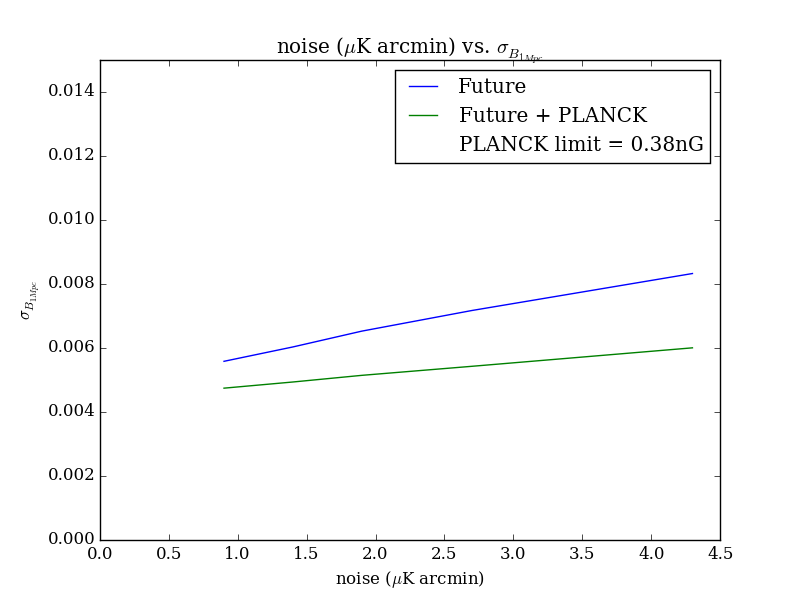
\includegraphics[scale=0.8]{images/noise.png}
\caption{Plot of noise vs experimental uncertainty on $B_{1Mpc}$. This plot shows that, as expected, reducing the nosie levels (adding more detectors) improves the constraints on $B_{1Mpc}$.}
\label{fig:noise}
\end{figure}

\begin{figure}[h]
\centering
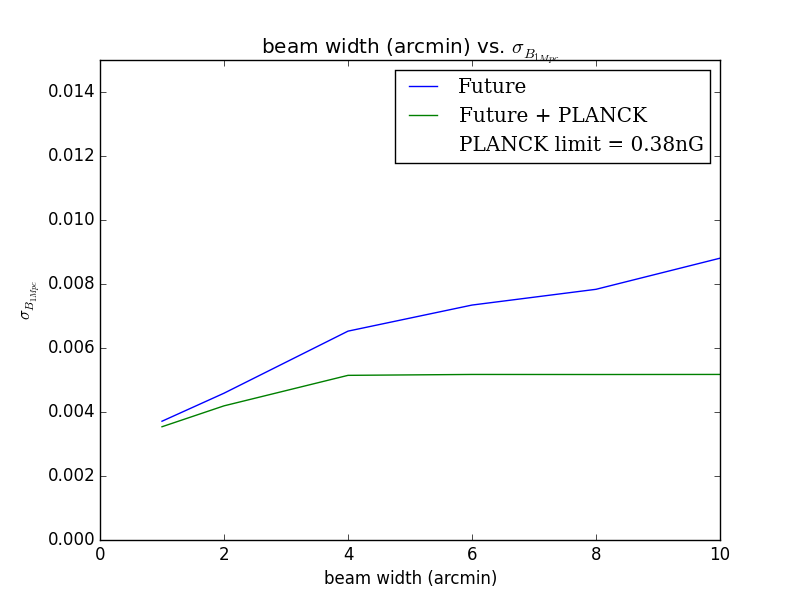
\includegraphics[scale=0.8]{images/width.png}
\caption{Plot of beam width vs the experimental uncertainty on $B_{1Mpc}$. This plot shows that refining the width of the beam reudces the uncertainty on $B_{1Mpc}$.}
\label{fig:width}
\end{figure}

\begin{figure}[h]
\centering
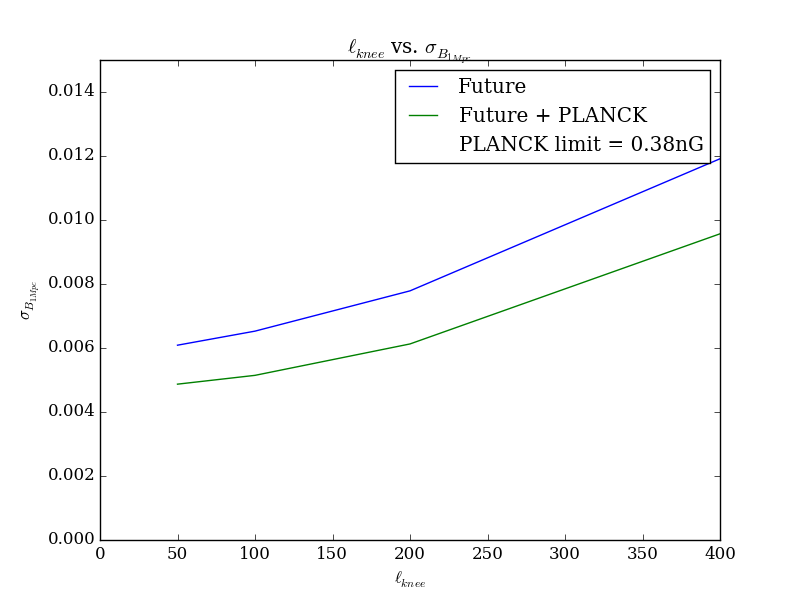
\includegraphics[scale=0.8]{images/knee.png}
\caption{Plot of $\ell_{knee}$ vs experimental uncertainty on $B_{1Mpc}$ with all other variables held fixed. This plot shows that precision on $B_{1Mpc}$ decreases as $\ell_{knee}$ increases, so it is best to reduce $\ell_{knee}$.}
\label{fig:knee}
\end{figure}

\begin{figure}[h]
\centering
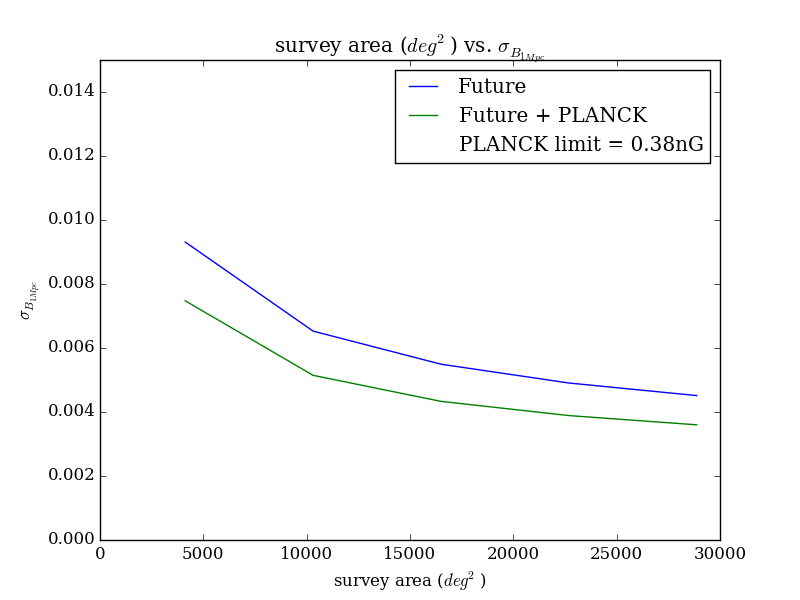
\includegraphics[scale=0.8]{images/area.png}
\caption{Plot of survey area vs the experimental uncertainty on $B_{1Mpc}$ with all other independent experimental variables held fixed. This plot shows that as the survey area of an experiment increases, the precision on $B_{1Mpc}$ improves, thus the ideal experiment for detecting PMFs will increase the survey area. The blue line shows the precision for Future CMB experiments on their own and the green line shows the same precisions when combined with the PLANCK data set.}
\label{fig:area}
\end{figure}

The forecasts for the next stages of CMB experiments are promising. Our current best limits from Planck are $\sigma(B_{1Mpc}) \geq 0.38nG$. In comparison, the limits from stage-3 and stage-4-like covariances fall within the range of $\sim$ 0.01nG to $\sim$ 0.001nG. In the most optimistic cases, measurements will have 100 times more sensitivity to PMFs than current experiments.

The optimal experimental design for detecting PMFs maximises the survey area and minimises the beam width, noise and $\ell_{knee}$. The sensitivity is independent of the beam and calibration uncertainties. 

As shown in figure~\ref{fig:area}, $\sigma(B_{1Mpc})$ decreases as the survey area increases. If we combine the mock covariances with PLANCK data our best constraints range from $\sigma(B_{1Mpc}) \geq 0.0075nG$ for a survey area of 4125 deg$^2$ to $\sigma(B_{1Mpc}) \geq 0.0036nG$ for a survey area of 28877 deg$^2$, improving by a factor of 2.08. We also see a factor of 1.28 improvement, when the noise decreases from 4.3 $\mu$K arcmin to 0.9 $\mu$K arcmin, yielding  $\sigma(B_{1Mpc}) \geq 0.0060nG$ and $\sigma(B_{1Mpc}) \geq 0.0048nG$ respectively, as seen in figure~\ref{fig:noise}. Decreasing the beam width from 10 arcmin to 1 arcmin improves sensitivity by a factor of 1.46 by reducing the uncertainty from $\sigma(B_{1Mpc}) \geq 0.0052nG$ to $\sigma(B_{1Mpc}) \geq 0.0035nG$ as per figure~\ref{fig:width}. In figure~\ref{fig:knee}, we see that a lower $\ell_{knee}$ improves sensitivity. At $\ell_{knee} = 50$, $\sigma(B_{1Mpc}) \geq 0.0049nG$ and in the worst-case scenario, when $\ell_{knee} = 400$, we have $\sigma(B_{1Mpc}) \geq 0.0096nG$ - a factor of 1.96 improvement. In contrast, changes to calibration and beam uncertainty have negligible effects on improving detection limits. For all values of beam and calibration uncertainties the sensitivity to the PMF strength is $\sigma(B_{1Mpc}) \geq 0.0051nG$.

\subsection{Parameter Constraints}

\begin{table}[h]
\centering
\caption{Mock Stage-3 and Stage-4 Variables}

\label{my-label}
\begin{tabular}{l|l|l}
\multicolumn{1}{c}{Variable} & \multicolumn{1}{|c}{Stage-3} & \multicolumn{1}{|c}{Stage-4} \\ \hline
\multicolumn{1}{c}{Survey area $(deg^2)$} & \multicolumn{1}{|c}{10313} & \multicolumn{1}{|c}{22689}  \\
\multicolumn{1}{c}{Noise ($\mu$K arcmin)} & \multicolumn{1}{|c}{2.7} & \multicolumn{1}{|c}{1.3}  \\
\multicolumn{1}{c}{$\ell_{knee}$} & \multicolumn{1}{|c}{100} & \multicolumn{1}{|c}{50} \\
\multicolumn{1}{c}{beam width (arcmin)} & \multicolumn{1}{|c}{4.0} & \multicolumn{1}{|c}{4.0}   \\
\multicolumn{1}{c}{calibration error (\% error)} & \multicolumn{1}{|c}{0.01} & \multicolumn{1}{|c}{0.01} \\
\multicolumn{1}{c}{beam uncertainty (\% error)} & \multicolumn{1}{|c}{0.05} & \multicolumn{1}{|c}{0.05}
\end{tabular}

\bigskip
\begin{flushleft}
This table shows the values for each variable for both the mock covariance matrices used in 
\end{flushleft}
\end{table}

\begin{figure}[h]
\centering
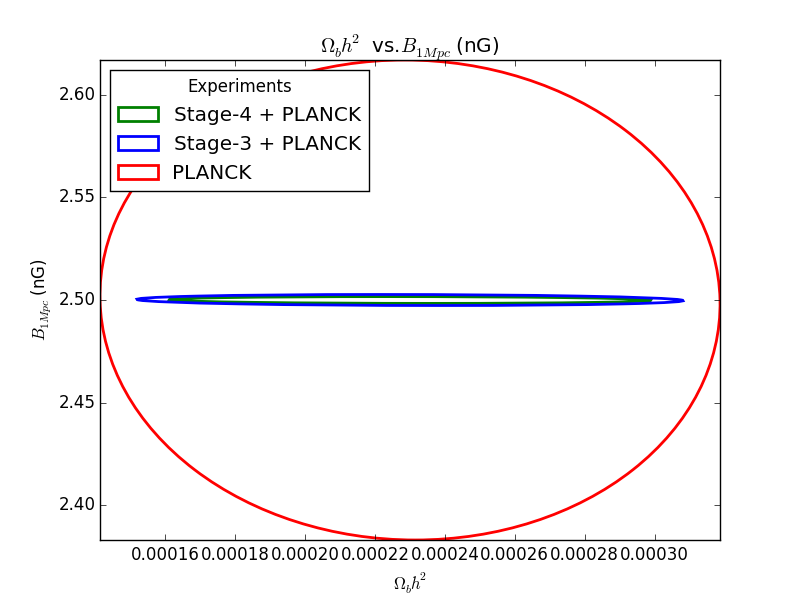
\includegraphics[scale=0.8]{images/contours/ombh.png}
\caption{}
\label{fig:ombh}
\end{figure}

\begin{figure}[h]
\centering
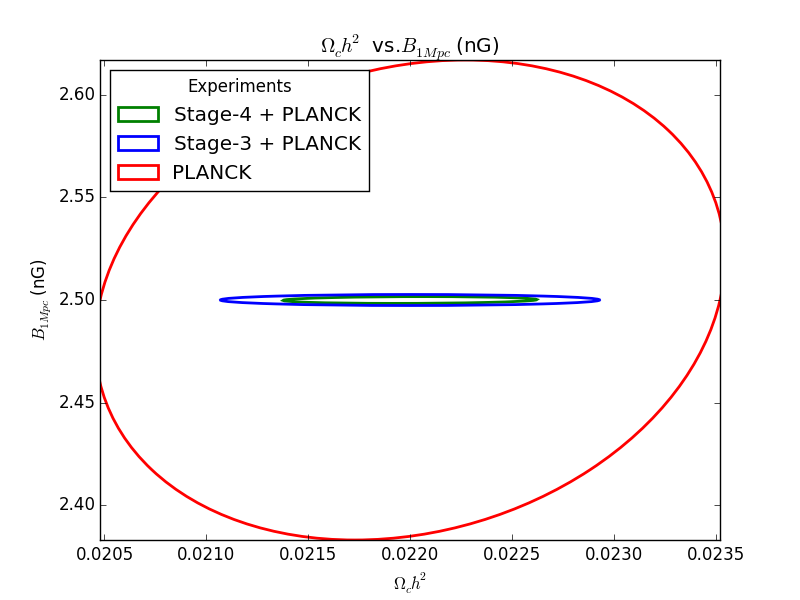
\includegraphics[scale=0.8]{images/contours/omch.png}
\caption{}
\label{fig:omch}
\end{figure}

\begin{figure}[h]
\centering
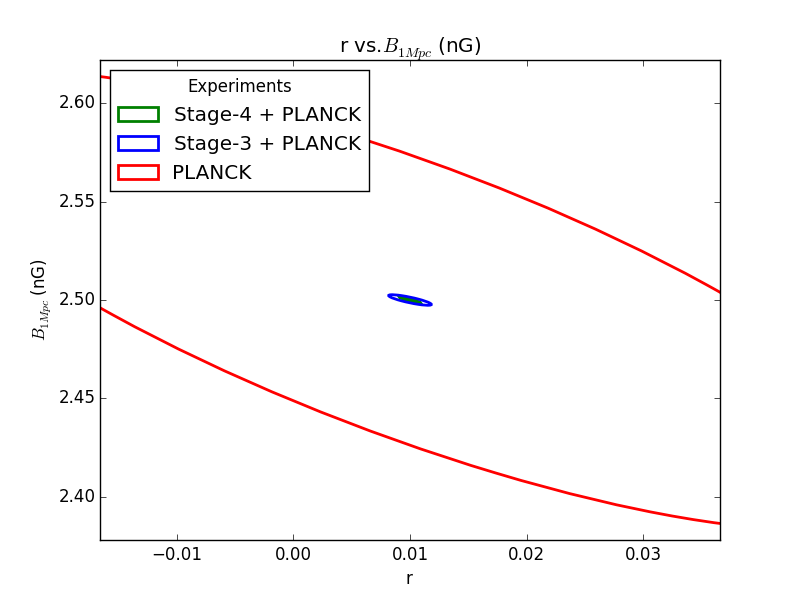
\includegraphics[scale=0.8]{images/contours/r.png}
\caption{}
\label{fig:r}
\end{figure}